\begin{align}
    \brak{\dfrac{5}{6}}^nu(n) &\zed \dfrac{1}{1-\dfrac{5}{6}z^{-1}} \quad \abs{z} > \frac{5}{6}
\\    \brak{\dfrac{6}{5}}^nu(-n-1) &\zed  
    = \dfrac{1}{\dfrac{6}{5}z^{-1}-1} \quad \abs{z} < \frac{6}{5}
\end{align}
Therefore, the Z transform of the given sequence is 
\begin{multline}
    \dfrac{1}{1-\dfrac{5}{6}z^{-1}}+\dfrac{1}{1-\dfrac{6}{5}z^{-1}}\label{ec/2005/6z}
= dfrac{2-\dfrac{61}{30}z^{-1}}{\brak{1-\dfrac{5}{6}z^{-1}}\brak{1-\dfrac{6}{5}z^{-1}}}
 \frac{5}{6} < \abs{z} < \frac{6}{5}
\end{multline}
See Fig. \ref{ec/2005/6plot}.
\begin{figure}
    \centering
    \resizebox{\columnwidth}{!}{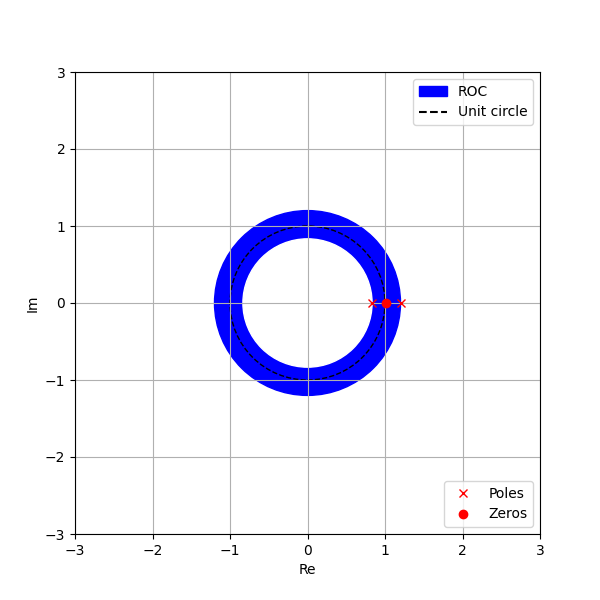
\includegraphics{solutions/ec/2005/6/figures/plot.png}}
    \caption{Pole-zero plot of the system}
    \label{ec/2005/6plot}
\end{figure}
